\section{Morphology and finite state techniques}
\begin{itemize}
	\item Morphology concerns the \textbf{structure of words}
	\item \textit{Morpheme}: minimal information carrying unit in a word. A word consists of morphemes
	\item \textit{Affix}: Morphemes that only occur in conjunction with other morphemes
	\item \textit{Stem}: a word is made up of a stem and zero or more affixes. Stems are therefore stand-alone morphemes
	\item There are different forms of affixes that describe when (prefix, suffix, infix, ...)
	\item An affix is productive if it applies in general and therefore also probably for new words
	\item \textbf{Inflectional morphology}
	\begin{itemize}
		\item Fills predefined slots in paradigm, as plural, tense,... (create different grammatical forms, but word stays the same)
		\item Fully productive, except irregular forms
		\item Inflectional affixes are not combined in English
	\end{itemize}
	\item \textbf{Derivational morphology}
	\begin{itemize}
		\item Forming a new word through affix (also change of meaning possible)
		\item May change POS tag
		\item Examples include \textit{anti-}, \textit{re-}, \textit{-ism}, \textit{-ist} (``reset'' vs. ``set'')
		\item Generally semi-productive (applies for only subset of words in language)
		\item Include \textit{zero-derivation}: word that is both verb and noun, e.g. ``text'' vs. ``(to) text (someone)''
	\end{itemize}
	\item Ambiguities in terms of morphemes (single stems or affixes are ambiguous like ``dog'') or structure (combination of affixes/stem like ``shorts'' vs ``short-s'')
	\item \textbf{Bracketing}
	\begin{itemize}
		\item Starting from the stem, find the combination of nearby affixes that still lead to a possible form
		\item Example \textit{un-ion-ise-ed}. Putting \textit{un-} and \textit{ion} together not possible as this forms a non-valid word (union would be different stem). $\Rightarrow$ \textit{un-(ion-ise)-ed}
		\item Next, adding the \textit{-ed} ending is valid, and finally concatenating it with \textit{un-}: \textit{(un-((ion-ise)-ed))}
	\end{itemize}
\end{itemize}
\subsection{Applications of morphological processing in NLP}
\begin{itemize}
	\item We can use morphology to create a full-form lexicon (lexicon with each form of every word in it). However, this tends to explode very fast (high redundancy) and is not scalable for new words
	\item \textbf{Stemming}: use rules to get the stem form of a word. This allows us to match words to a small set of base words
	\item \textbf{Lemmatization}: Only finding split of stems and affixes. Is the preprocessing step before parsing (understanding the word!)
	\item Morphological process can either by analysis or generation
	\item Possible aspects/steps of morphological processing
	\begin{enumerate}
		\item Surface/ground-word mapped to stem(s) and affixes. Either by declaring the affixes (\textit{ping-ed}) or by explicitly saying which rule was applied (\textit{ping} \textit{PAST\_VERB})
		\item After knowing the affixes, analyze internal structure by bracketing
		\item Finally, understand syntactic and semantic effects where parsing can filter results of previous stages
	\end{enumerate}
	\item Overall, we need a lexicon combining three aspects:
	\begin{itemize}
		\item affixes (with the associated information they carry)
		\item irregular forms
		\item stems (with syntactic categories)
	\end{itemize}
\end{itemize}
\subsection{Spelling rules}
\begin{itemize}
	\item English morphology is essentially concatenative
	\item English spelling rules can be described independently of the particular stems and affixes involved. It simply looks at the affix boundaries.
	\item Example spelling rule for e-insertion:
	$$\epsilon \to \text{e}/\left\{\begin{array}{c}
	\text{s}\\
	\text{x}\\
	\text{z}
	\end{array}\right\}\hat{\text{ }}\textunderscore s$$
	Here, the formula is interpreted as ``an empty string maps to e if an s,x or z is followed by an s of the next affix'' (where e is inserted in the underscore space)
	\item Finite state machines (or transducers also creating corresponding output while parsing) can be used to implement spelling rules
	\begin{figure}[ht]
		\centering
		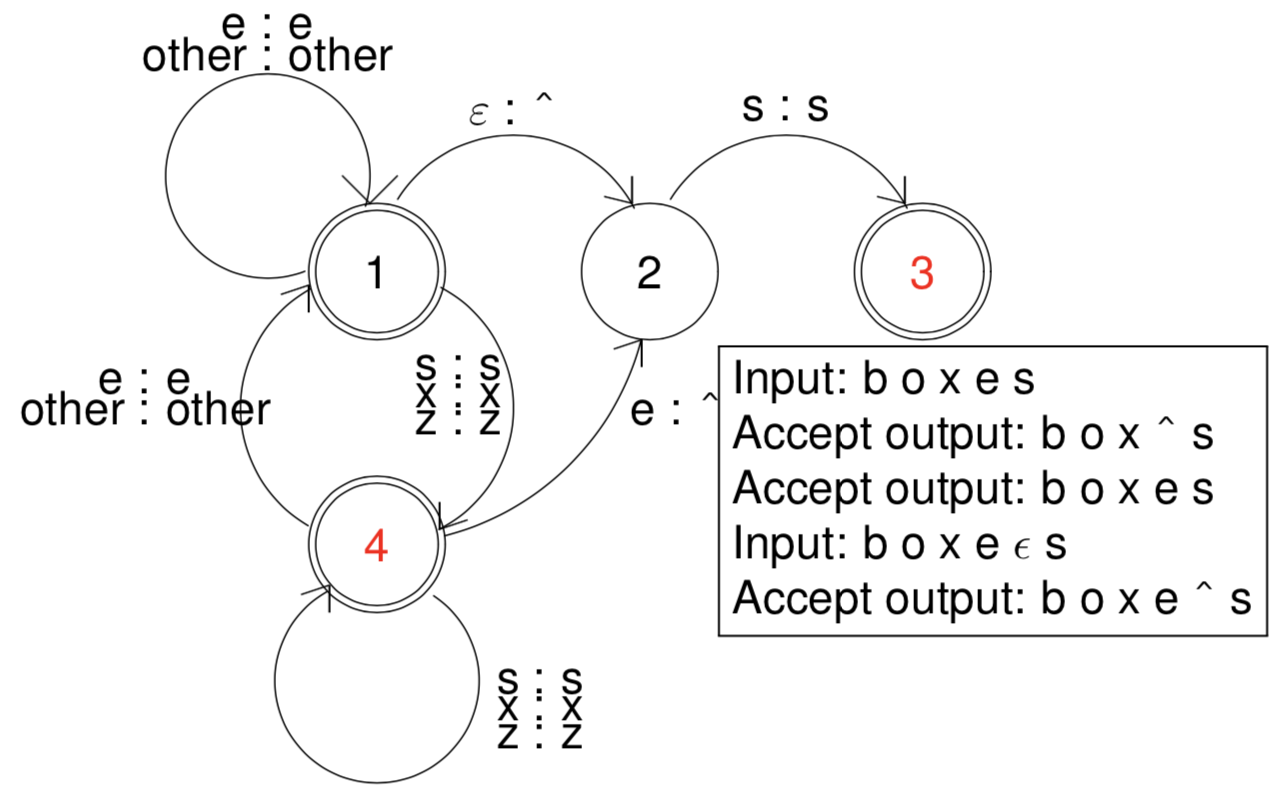
\includegraphics[width=0.4\textwidth]{figures/morphology_FST.png}
	\end{figure}
	\item Each transition corresponds to a pair of characters. 
	\item When the transducer is run in analysis mode, the system can detect an affix boundary (where we look up the stem and affix in the corresponding lexicon)
	\item In generation mode, we can just put in our parsed version and generate the correct spelling
	\item Morphology systems are usually implemented so that there is one FST per spelling rule and these operate in parallel
	\item However, FST are not applicable for internal structures as for example no bracketing model is possible
	\item A system which generates invalid output/accepts invalid derivations is said to \textbf{overgenerate}.
\end{itemize}